\documentclass[11pt,leqno]{article}

\usepackage{amssymb}
\usepackage{amsmath}
\usepackage{mathrsfs}
\usepackage{xcolor}
\usepackage{mathrsfs}
\usepackage{hyperref}
\usepackage{comment}
\usepackage{graphicx}
\graphicspath{ {./} }

\textwidth              16 cm
\textheight             24.5  cm
\oddsidemargin          -1   cm
\evensidemargin         -1cm
\topmargin              -1 cm
\setlength{\evensidemargin}{15.5pt}
\setlength{\oddsidemargin}{2.5pt}

\pagestyle{empty}

\def\ClasaO{{\mathcal O}}

\usepackage{algpseudocode}

\title{Tema 1}
\author{Mihai Cristian-Laurentiu 2B4, Stamate Valentin 2B4}
\date{06.11.2020}

\begin{document}

\maketitle


1. Pentru a putea raspunde la intrebare trebuie sa calculam numarul de componente conexe din graful G. In cazul in care numarul componentelor conexe din G este mai mic sau egal decat k, raspunsul este Da, altfel Nu. Vom folosi algoritmul DFS cu liste de adiacenta.
\vspace{0.5cm}
\begin{algorithmic}
    \State //vizitat initializat cu 0
    \State $ NC \gets 0 $;
    \For{($ i = \overline{1, n} $)}
            \If{($ !vizitat[i] $)}
                \State $ DFS(i) $;//$\ClasaO(n+m)$ ,DFS aplicat in graful G din nodul i;
                \State $ NC \gets NC+1 $;// numarul componentelor conexe ;
            \EndIf
    \EndFor
    \If{($ k>=NC $)}
        \State $ printf("DA") $;
    \Else
        \State $ printf("NU") $;
    \EndIf
\end{algorithmic}

\vspace{0.5cm}

2.
a) Din enuntul problemei stim ca fiecare doi utilizatori au exact o cunostinta comuna. Aceasta proprietate determina ca drumul minim dintre doua noduri sa fie cel mult de lungime 2, cu alte cuvinte $ d(G)=2 $.
Presupunem prin reducere la absurd ca exista un circuit de lungime 4. Pentru existenta unui astfel de circuit ar trebui sa existe mai mult de un vecin comun intre doua noduri. Contradictie, oricare doua noduri au exact un vecin comun . In concluzie nu exista circuite de lungime 4 in graful G.
\begin{center}
    \centerline{
        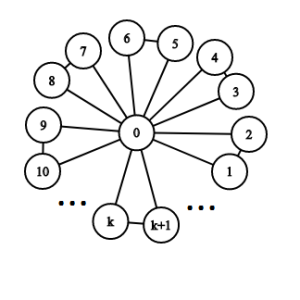
\includegraphics[scale=0.70]{graf_ex2.png}
    }
\end{center}

b) Pentru a arata aceasta proprietate vom folosi reprezentarea grafului. Observam ca v impreuna cu orice vecin al face parte dintr-o 3-clica, insa putem distinge doua cazuri:

\begin{itemize}
    \item cand v este un nod din margine (observabil pe reprezentarea grafica) acesta are exact 2 vecini ($d_G(v)=2$) formand cu acestia o 3-clica ($[{v} \cup N_G(v)]$) care are 3 muchii, deci se respecta proprietatea: $3d_G(v)/2=3*2/2=3$ muchii.
    \item cand v este nodul din mijloc care face parte din toate 3-clicile din graful G,  $d_G(v)=n-1$ ,unde n este numarul de noduri. Observam ca numarul de 3-clici care se formeaza este  $k=(n-1)/2$  deci numarul de muchii din aceste clici(o 3-clica are 3 muchii) este: \\$3k=3(n-1)/2=3*d_G(v)/2$, ceea ce trebuia aratat.
\end{itemize}
c)Plecand tot cu aceeasi idee de la punctul b observam ca nodul din mijloc este adiacent cu toate celelate noduri,  $d_G(v)=n-1$ fapt mentionat anterior, deci nu putem distinge doua cazuri. Astfel singurele noduri care pot fi neadiacente sunt nodurile care fac parte din 3-clici diferite. Fie $A,B$ doua 3-clici diferite din $G(V,E)$ , $u \in A , v \in B$,u,v neadiacente , stiind ca ambele noduri fac parte din 3-clici $d_A(u)=d_B(v)=2$. 
In concluzie oricare doua noduri neadiacente fac parte din  3-clici diferite deci au gradul 2, cu alte cuvinte, au acelasi numar de vecini.

\vspace{0.5cm}

3. 
Observam ca putem imparti drumul in doua segmente: primul in urcare iar celalalt in coborare. Deoarece pentru primul drum studentul trebuie doar sa urce, multimea drumurilor de acest fel formeaza un subgraf aciclic, deoarece arcele sunt orientate de la nodurile cu inaltime mai mica la nodurile cu inaltime strict mai mare.
Acelasi lucru se intampla si pentru drumul de coborare. Astfel putem folosi ordonarea topologica impreuna cu algoritmul pentru determinarea drumurilor de cost minim pentru un $dag$, prezentate in curs.
Ruland algoritmii pentru ambele subgrafuri vom obtine costul minim de la fiecare nod disponibil la punctul de start, respectiv punctul de oprire. Avand cei doi vectori de cost minim putem alege nodul care 
se afla in ambele subgrafuri si are suma minima a costului dintre cele doua drumuri. Observam ca putem pleca cu construirea drumurilor minime din nodul destinatie deoarece "strada" se poate parcurge in ambele sensuri.

\vspace{0.5cm}
\begin{algorithmic}
    \State $G_u = buildDAG(G, start, alt)$
    \State $G_d = buildDAG(G, dest, alt)$
    \\
    \State $T_u = topological(G_u)$
    \State $T_d = topological(G_d)$
    \\
    \State $minimimCost(T_u, prev_u, cost_u)$
    \State $minimimCost(T_d, prev_d, cost_d)$
    \\
    \State $final\_cost \gets INF$
    \\ cautarea nodului
    \For {$ i \gets 1, n $}
        \If {$ cost_u[i] != INF \; and \; cost_d[i] != INF $}
            \If {$ cost_u[i] + cost_d[i] < final\_cost $}
                \State $final\_cost = cost_u[i] + cost_d[i]$
                \State $u = i$
            \EndIf
        \EndIf
    \EndFor
    \\// construirea drumului
    \State $i = u$
    \While {$i != start$}
        \State $drum.push\_first(i)$ // pune nodul i pe prima pozitie
        \State $i = prev\_u[i]$
    \EndWhile
    \\
    \State $i = u$
    \While {$i != start$}
        \State $drum.push\_back(i)$ // pune nodul i pe ultima pozitie
        \State $i = prev\_v[i]$
    \EndWhile 
    \\
    \State $print(drum)$

\end{algorithmic}

a. Constructia subgrafului o vom face printr-o parcurgere $DFS$ punand conditia ca fiecare vecin sa aiba inaltimea strict mai mare decat nodul de start respectiv oprire. Folosind algoritmul de mai sus
putem determina un astfel de drum in $\ClasaO(n + m)$.

b. Acelasi procedeu ca si la subpunctul a punand conditia ca fiecare vecin sa aiba inaltimea mai mare sau egala cu cea a nodului dat. Complexitatea ramane $\ClasaO(n + m)$

\vspace{0.5cm}

4. Avem urmatoarele proprietati:
\begin{itemize}
    \item Se stie ca, avand cele doua partitii A si B ale lui G orice drum intre doua noduri din A, respectiv din B in $T_s$ este minim.
    \item Cei doi subarbori $T_s^1$ si $T_s^2$ sunt subarbori in $SP-arborele \; T_{s'}$ asociat tripletei $(G - e, \alpha, s)$. 
    Demonstratie: Fie $x, y \in A, A \in V(G - e), e \cap E(T_s^1) = \emptyset$ si P' un xy-drum in arborele $T_s^1$ si $P''$ un drum in $T_s$ astfel incat $V(P')=V(P'')$. Presupunand ca $\alpha(P') < \alpha(P'')$ vom obtine o contradictie cunoscand deja ca $P''$ este un drum de cost minim. 
    Astfel drumul cel mai mic de la x la y in $T_{s'}$ este chiar $P'$. 
    Cum aceste drumuri care sunt minime in $T_{s'}$ formeaza subarborele $T_s^1$ resulta ca $T_s^1$ este subarbore in $T_{s'}$. Analog se poate demonstra pentru subarborele $T_s^2$.
\end{itemize}

a. Un su-drum de cost minim $ \subseteq E(T_s^1), s, u \in A$ impreuna cu ipotezele 1 si 2 stim ca $T_s^1$ este subarbore in $T_{s'}$ si in $T_s$, atunci un su-drum de cost minim care se afla in $G - e$ este minim si in $G$. 

b. La fel cum am aratat la subpunctul a, folosindu-ne de ipotezele 1 si 2 stim ca un $vt-drum$ de cost minim $ \subseteq E(T_s^2), v, t \in B$ este subarbore in $T_{s'}$ dar si in $T_s$. Atunci un vt-drum de cost minim care se afla in $G - e$ este minim si in $G$.

c. Deoarece stim ca $T_s^1$ si $T_s^2$ sunt subarbori in $T_{s'}$, iar din G este stearsa doar o muchie, atunci cei doi subarbori vor fi uniti doar printr-o singura muchie $m \in F, m\; != e$ formand SP-arborele asociat tripletei $(G - e, \alpha, s)$.
Acest lucru este usor de demonstrat deoarece daca cei doi subarbori ar fi uniti prin mai mult de o muchie s-ar forma un ciclu ceea ce ar contrazice proprietatea de arbore.

d. Este cunoscut faptul ca orice su-drum $s, u \in A$ este minim in $G - e$ intrucat $T_1$ este subarbore in $T_{s'}$. Acelasi lucru se intampla si pentru un vt-drum unde $v, t \in B$ iar $T_s^2$ este subarbore in $T_{s'}$.
Se observa imediat faptul ca luand o muchie din F cu capetele in u si v, ea va uni cei doi arbori $T_s^1$ si $T_s^2$ formand $T_{s'}$. Astfel un st-drum din $T_{s'}$ va traversa cei doi subarbori printr-o singura muchie astfel drumul putand fi impartit in 3:
prima si a treia parte vor trece prim $T_s^1$ respectiv $T_s^2$ iar a doua este muchia care uneste subarborii. Astfel costul unui st-drum va fi egal cu $min[\alpha_G(s, u) + \alpha_{uv} + \alpha_G(v, t)]$, ceea ce trebuia aratat.

e. Pentru a determina costul minim al unui st-drum in $G - e$ putem folosi algoritmul lui Dijkstra cu o coada de prioritate pornind de la nodul s. Complexitatea algoritmului este $\ClasaO(m + nlogn)$.

\end{document}
